\section{Wymagania wstępne}
System do prawidłowego działania od strony klienckiej wymaga zainstalowanej aktualnej wersji przeglądarki Firefox (co najmniej wersja 20), Chrome (co najmniej wersja 27) lub Internet Explorer (w wersji 9 lub wyżej) z włączoną obsługą Javascript. Po wejściu na stronę użytkownik, aby przejść dalej, musi podać swoje dane, żeby się zalogować. W przypadku, gdy nie posiada jeszcze konta, powinien zarejestrować się w systemie.
\begin{figure}[H]
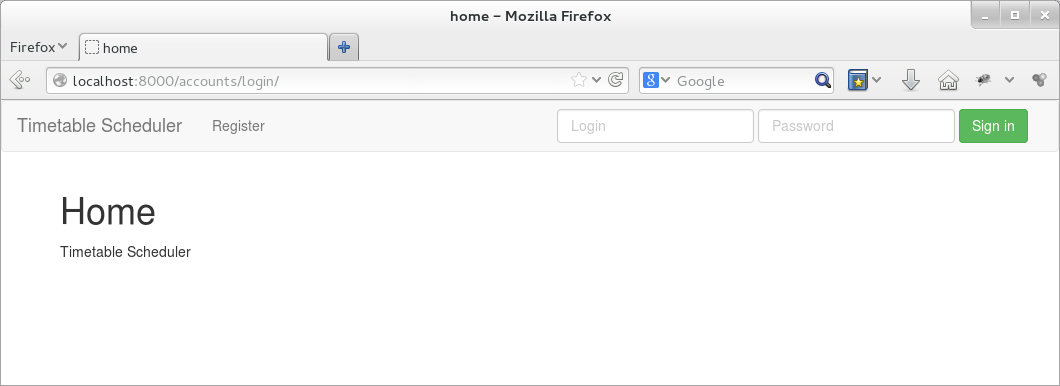
\includegraphics[width=15cm]{img/guide/user1.png}
\caption{Logowanie do systemu}
\end{figure}

\par Po zalogowaniu użytkownik uzyskuje dostęp do dwóchb głównych funkcjonalności systemu: dodawania nowego zadania wygenerowania planu, lub podejrzenia dodanych zadań.

\begin{figure}[H]

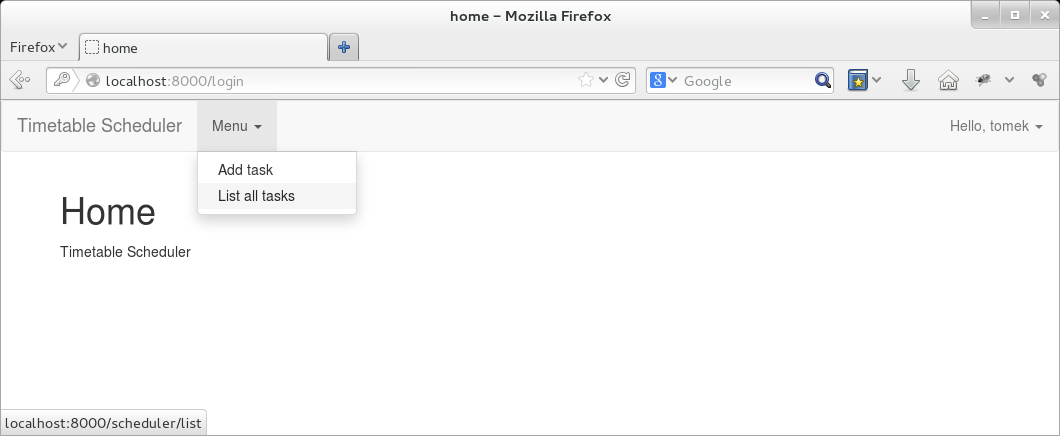
\includegraphics[width=15cm]{img/guide/user3.png}
\caption{Menu główne}
\end{figure}

\par Formularz dodawania zadania wymaga od użytkownika wybór algorytmu z listy dostępnych algorytmów, ustalenie limitu czasowego na zadanie i wybrania z plików dostępnych na dysku twardym użytkownika pliku z definicją problemu.

\begin{figure}[H]
\centering
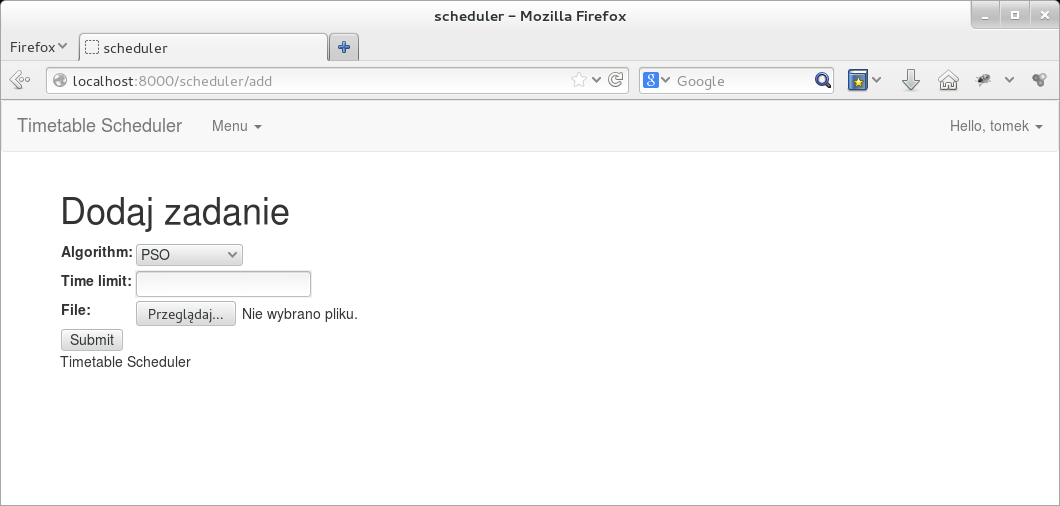
\includegraphics[width=15cm]{img/guide/user4.png}
\caption{Formularz dodawania nowego zadania}
\end{figure}
\par Dodane w ten sposób zadanie pojawia się na liście zadań. Użytkownik widzi dla każdego zadania wybrany algorytm, limit czasowy, czas rozpoczęcia zadania, czas do ukończenia i status wykonywania zadania. Dodatkowo dla każdego zadania można przejść do szczegółów zadania. Dla zadań ukończonych możliwe jest również usunięcie zadania.

\begin{figure}[H]
\centering
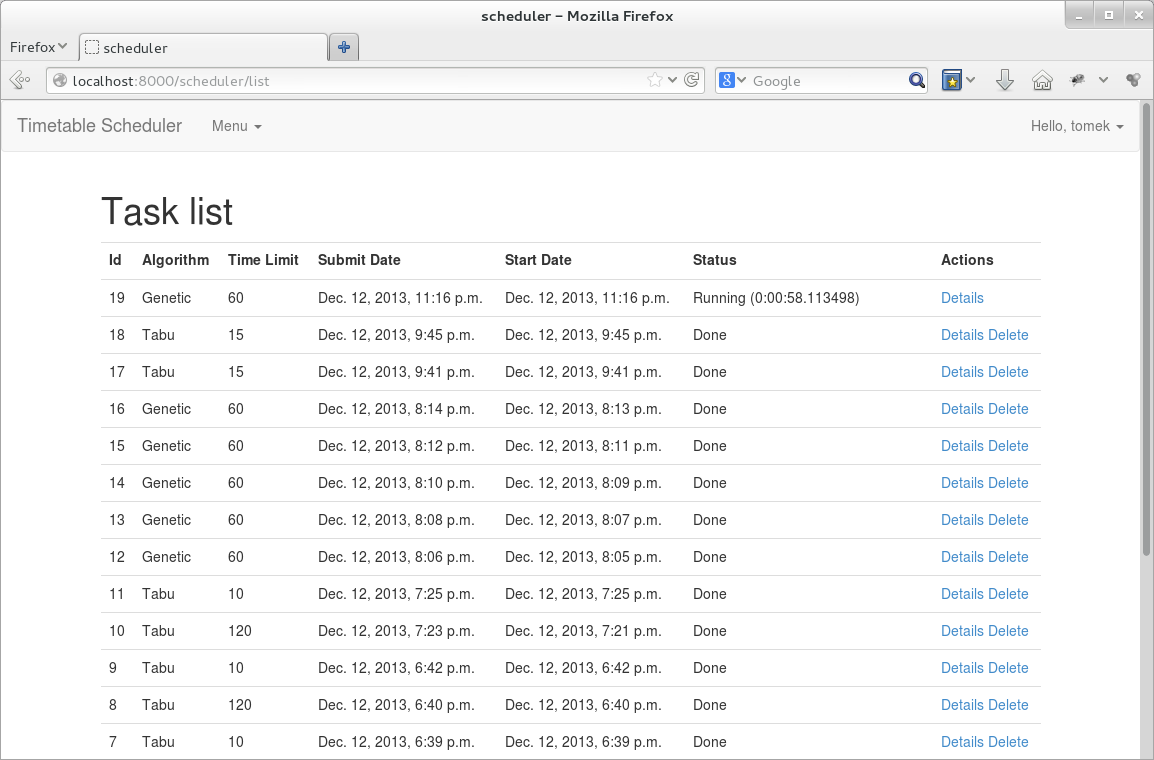
\includegraphics[width=13cm]{img/guide/user5.png}
\caption{Widok listy zadań}
\end{figure}


\par Widok szczegółów zadania prezentuje użytkownikowi listę wszystkich programów nauczania zdefiniowanych w pliku z ograniczeniami. Dla każdego programu nauczania dostępny jest link do widoku planu zajęć.
\begin{figure}[H]
\centering
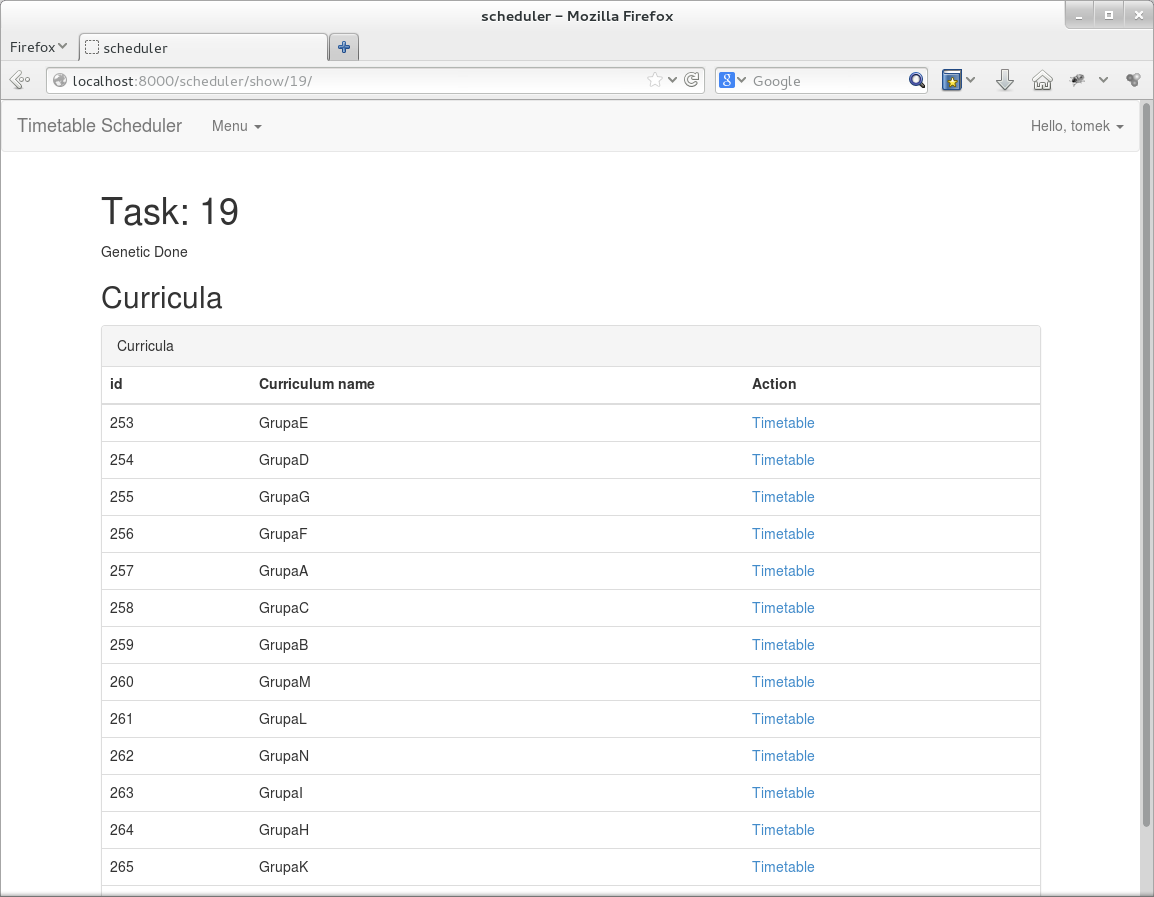
\includegraphics[width=12cm]{img/guide/user6.png}
\caption{Widok listy programów nauczania}
\end{figure}

\par Widok wygenerowanego planu zajęć dla programu nauczania zawiera komponent kalendarza, który prezentuje wygenerowany plan zajęć w odniesieniu do bieżącego tygodnia. Dla każdej godziny lekcyjnej w planie użytkownik może podejrzeć jej szczegóły: godzinę rozpoczęcia i zakończenia i przydzieloną salę.
\begin{figure}[H]
\centering
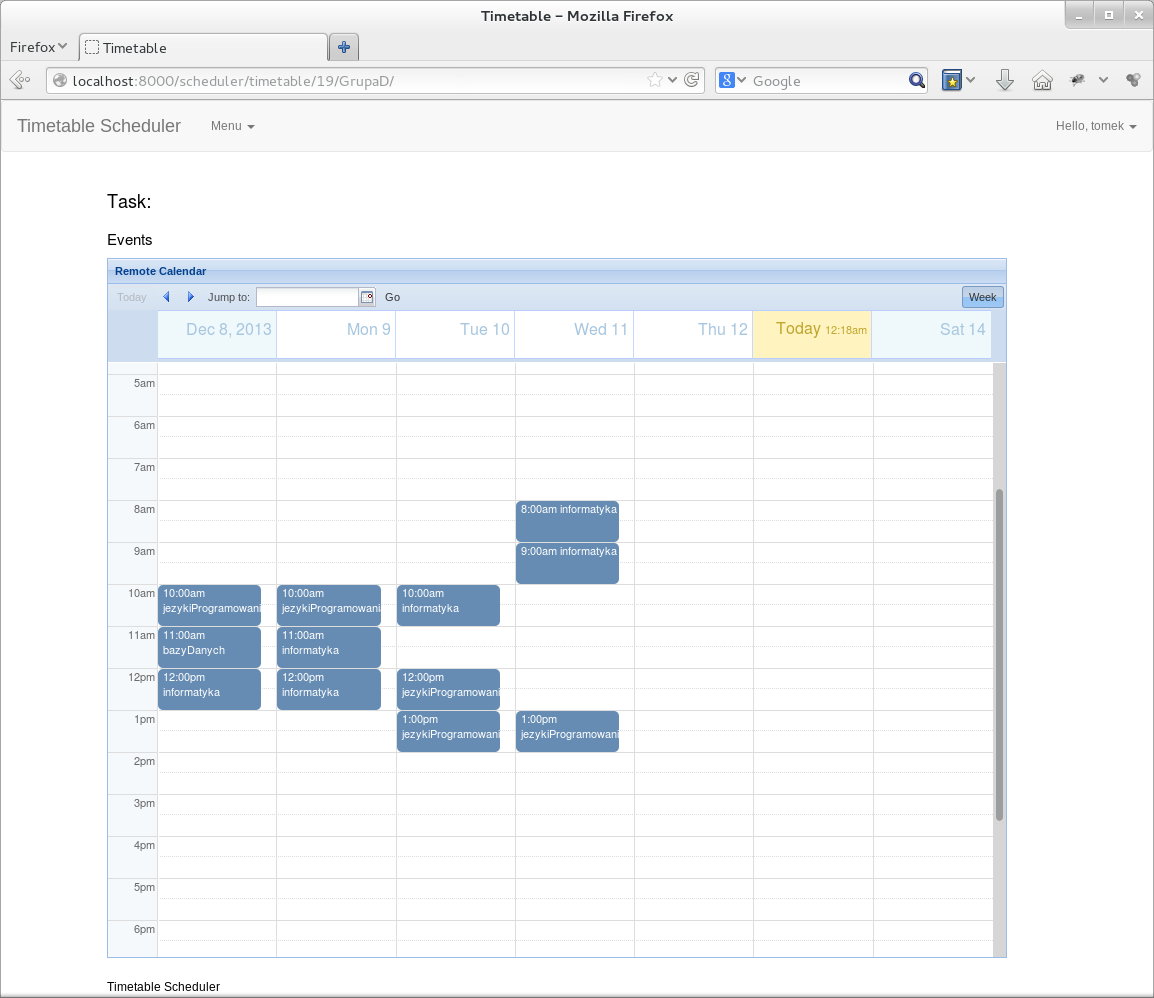
\includegraphics[width=13cm]{img/guide/user7.png}
\caption{Widok kalendarza z ułożonym planem}
\end{figure}
\begin{figure}[H]
\centering
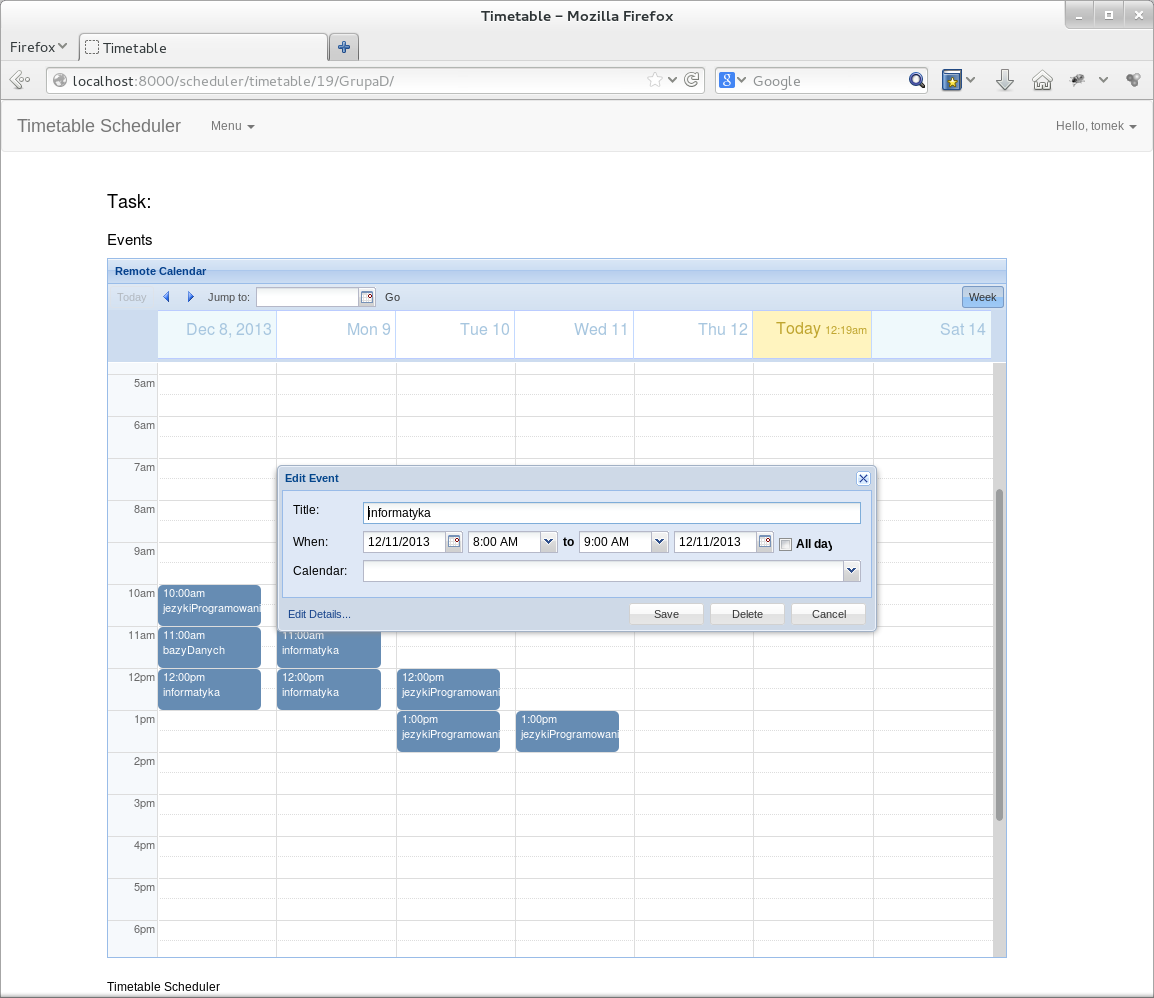
\includegraphics[width=13cm]{img/guide/user9.png}
\caption{Widok szczegółów wydarzenia}
\end{figure}